%&<latex>
\documentclass[letterpaper,12pt]{article}
\pdfoutput=1

%%%%%%%%%%%%%%%%%%%%%%%%%%%%%%%%%%%%%%%%%%%%%%%%%%%%%%%%%%%%
%% preamble %%%%%%%%%%%%%%%%%%%%%%%%%%%%%%%%%%%%%%%%%%%%%%%%
\pdfpagewidth = 8.5in
\pdfpageheight = 11.0in
\usepackage[left=1in,right=1in,top=1in,bottom=1in]{geometry}

\pagestyle{plain}
\pagenumbering{arabic}
\usepackage[nodisplayskipstretch]{setspace}
\usepackage[fleqn]{amsmath}
\usepackage{amssymb}
\usepackage{graphicx}
\usepackage[hyphens]{url}
\usepackage{verbatim}
\usepackage[title]{appendix}
\usepackage{indentfirst}
\usepackage{booktabs}
\usepackage{multirow}
\usepackage{ragged2e}
\usepackage{upgreek}
\usepackage[T1]{fontenc}
\usepackage[titles]{tocloft}
\usepackage{xspace}
% xcolor allows rowcolors for tables
\usepackage[table,x11names,dvipsnames,table]{xcolor}
% \usepackage[usenames]{color}
\usepackage{ifthen}
\usepackage{cancel}
\usepackage{array}
\usepackage{tabulary}
\usepackage{authblk}
\usepackage{tikz}
\usepackage{pdflscape}
\usepackage[normalem]{ulem}

%% Set up color palettes %%%%%%%%%%%%%%%%%%%%%%%%%%%%%%%%%%%%%%%%%%%%
% Color palette GreenOrange_6 from
% https://jiffyclub.github.io/palettable/tableau/
\definecolor{pgreen}     {RGB}{50,162,81}
\definecolor{porange}    {RGB}{255,127,15}
\definecolor{pblue}      {RGB}{60,183,204}
\definecolor{pyellow}    {RGB}{255,217,74}
\definecolor{pteal}      {RGB}{57,115,124}
\definecolor{pauburn}    {RGB}{184,90,13}
%%%%%%%%%%%%%%%%%%%%%%%%%%%%%%%%%%%%%%%%%%%%%%%%%%%%%%%%%%%%%%%%%%%%%
\definecolor{mygray}{gray}{0.9}

\usepackage{hyperref}
\hypersetup{pdfborder={0 0 0},
            colorlinks=true,
            % colorlinks=false,
            urlcolor=porange,
            linkcolor=pauburn,
            citecolor=pteal}

\usepackage[capitalize]{cleveref}
\newcommand{\crefrangeconjunction}{--}

% Set up line numbering; using lineno to number lines of paragraphs with
% equations sanely
\usepackage[right, mathlines]{lineno}
\setlength\linenumbersep{1cm}
\def\linenumberfont{\normalfont\scriptsize\sffamily}

% Set up caption formatting
\usepackage{subcaption}
\usepackage[format=plain, labelsep=period, singlelinecheck=false, skip=4pt, font=sf]{caption}
\DeclareCaptionLabelFormat{noSpace}{{#1}{#2}}
\DeclareCaptionListFormat{figList}{Figure {#2}.}
\DeclareCaptionListFormat{sFigList}{Figure S{#2}.}

\newenvironment{mytitle}
 {\parskip=0pt\par\nopagebreak\centering\LARGE\slshape}
 {\par\noindent\ignorespacesafterend}

% Define tightly formated list environments via enumitem
\usepackage{enumitem}
\newenvironment{tightItemize}{%
\begin{itemize}[noitemsep, topsep=0pt, parsep=0pt, partopsep=0pt]}
{\end{itemize}}

\newenvironment{veryTightItemize}{%
\begin{itemize}[noitemsep, topsep=0pt, parsep=0pt, partopsep=0pt, leftmargin=*]}
{\end{itemize}}

\newenvironment{tightEnumerate}{%
\begin{enumerate}[noitemsep, topsep=0pt, parsep=0pt, partopsep=0pt]}
{\end{enumerate}}

\newenvironment{veryTightEnumerate}{%
\begin{enumerate}[noitemsep, topsep=0pt, parsep=0pt, partopsep=0pt, leftmargin=*]}
{\end{enumerate}}

% Redefine abstract environment as a list to control left/right margins
% From https://tex.stackexchange.com/a/151589
\renewenvironment{abstract}
 {\small
  \begin{center}
  \bfseries \abstractname\vspace{-.5em}\vspace{0pt}
  \end{center}
  \list{}{%
    \setlength{\leftmargin}{5mm}%
    \setlength{\rightmargin}{\leftmargin}%
  }%
  \item\relax}
 {\endlist}

% \newcommand{\jedit}[2]{\sout{#1}{\color{red}{#2}}}
\newcommand{\jedit}[2]{#2}
\newcommand{\jcomment}[1]{({\color{pgreen}{JRO's comment:}} \textbf{\color{pgreen}{#1}})}

\newcommand{\citationNeeded}{\textcolor{magenta}{\textbf{[CITATION NEEDED]}}\xspace}
\newcommand{\tableNeeded}{\textcolor{magenta}{\textbf{[TABLE NEEDED]}}\xspace}
\newcommand{\figureNeeded}{\textcolor{magenta}{\textbf{[FIGURE NEEDED]}}\xspace}
\newcommand{\highLight}[1]{\textcolor{magenta}{\MakeUppercase{#1}}}

\newcommand{\fig}{Figure\xspace}
\newcommand{\figs}{Figures\xspace}
\newcommand{\tbl}{Table\xspace}
\newcommand{\tbls}{Tables\xspace}

\newcommand{\datasets}{data sets\xspace}
\newcommand{\dataset}{data set\xspace}

\newcommand{\ignore}[1]{}
\newcommand{\addTail}[1]{\textit{#1}.---}
\newcommand{\super}[1]{\ensuremath{^{\textrm{#1}}}}
\newcommand{\sub}[1]{\ensuremath{_{\textrm{#1}}}}
\newcommand{\dC}{\ensuremath{^\circ{\textrm{C}}}}
\newcommand{\tn}{\tabularnewline}
\newcommand{\spp}[1]{\textit{#1}}

\providecommand{\e}[1]{\ensuremath{\times 10^{#1}}}

\newcommand{\change}[2]{{\color{red} #2}\xspace}
\newcommand{\thought}[1]{\textcolor{purple}{THOUGHT: #1}}

\newcommand{\widthFigure}[5]{\begin{figure}[htbp]
\begin{center}
    \includegraphics[width=#1\textwidth]{#2}
    \captionsetup{#3}
    \caption{#4}
    \label{#5}
    \end{center}
    \end{figure}}

\newcommand{\heightFigure}[5]{\begin{figure}[htbp]
\begin{center}
    \includegraphics[height=#1\textheight]{#2}
    \captionsetup{#3}
    \caption{#4}
    \label{#5}
    \end{center}
    \end{figure}}

\newcommand{\smartFigure}[5]{%
    \begin{figure}[htbp]
        \begin{center}
            \includegraphics[width=\textwidth,height=#1\textheight,keepaspectratio]{#2}
            \captionsetup{#3}
            \caption{#4}
            \label{#5}
        \end{center}
    \end{figure}
}

\newcommand{\mFigure}[4]{\smartFigure{#1}{#2}{listformat=figList}{#3}{#4}\clearpage}
\newcommand{\embedHeightFigure}[4]{\heightFigure{#1}{#2}{listformat=figList}{#3}{#4}}
\newcommand{\embedWidthFigure}[4]{\widthFigure{#1}{#2}{listformat=figList}{#3}{#4}}
\newcommand{\siFigure}[4]{\smartFigure{#1}{#2}{name=Figure S, labelformat=noSpace, listformat=sFigList}{#3}{#4}\clearpage}

%% macro to make long strings breakable over lines
\makeatletter
\def\breakable#1{\xHyphen@te#1$\unskip}
\def\xHyphen@te{\@ifnextchar${\@gobble}{\sw@p{\allowbreak{}\xHyphen@te}}}
% \def\xHyphen@te{\@ifnextchar${\@gobble}{\sw@p{\hskip 0pt plus 1pt\xHyphen@te}}}
\def\sw@p#1#2{#2#1}
\makeatother

\newcommand{\given}{\ensuremath{\,|\,}\xspace}
\newcommand{\pr}{\ensuremath{p}}

\newcommand{\data}{\ensuremath{D}\xspace}
\newcommand{\model}[1][]{\ensuremath{M_{#1}}\xspace}
\newcommand{\parameters}[1][]{\ensuremath{\Theta_{#1}}\xspace}
\newcommand{\parameter}[1][]{\ensuremath{\theta_{#1}}\xspace}
\newcommand{\diff}[1]{\ensuremath{\mathrm{d}#1}}

\newcommand{\distgamma}{\ensuremath{\textrm{Gamma}}\xspace}
\newcommand{\distexponential}{\ensuremath{\textrm{Exponential}}\xspace}
\newcommand{\distbeta}{\ensuremath{\textrm{Beta}}\xspace}
\newcommand{\dgamma}[2]{\ensuremath{\distgamma(\textrm{shape} = #1, \textrm{mean} = #2)}}
\newcommand{\dexponential}[1]{\ensuremath{\distexponential(\textrm{mean} = #1)}}
\newcommand{\dbeta}[2]{\ensuremath{\distbeta(\alpha = #1, \beta = #2)}}

\newcommand{\ncomparisons}{\ensuremath{\mathcal{N}}\xspace}
\newcommand{\nevents}[1][]{\ensuremath{k_{#1}}\xspace}
\newcommand{\nexistingcats}{\ensuremath{\mathcal{K}}\xspace}
\newcommand{\nloci}[1][]{\ensuremath{m_{#1}}\xspace}

\newcommand{\observedallelecount}[1][]{\ensuremath{n_{#1}}\xspace}
\newcommand{\observedredallelecount}[1][]{\ensuremath{r_{#1}}\xspace}

\newcommand{\nodeallelecount}[2]{\ensuremath{n_{#1}^{#2}}}
\newcommand{\noderedallelecount}[2]{\ensuremath{r_{#1}^{#2}}}

\newcommand{\allelecount}[1][]{\ensuremath{\nodeallelecount{#1}{}}\xspace}
\newcommand{\redallelecount}[1][]{\ensuremath{\noderedallelecount{#1}{}}\xspace}

\newcommand{\leafallelecounts}[1][]{\ensuremath{\mathbf{n}_{#1}}\xspace}
\newcommand{\leafredallelecounts}[1][]{\ensuremath{\mathbf{r}_{#1}}\xspace}
\newcommand{\maxleafallelecounts}{\ensuremath{\textrm{max}(\mathbf{n})}\xspace}

\newcommand{\comparisondata}[1][]{\ensuremath{D_{#1}}\xspace}
\newcommand{\alldata}[1][]{\ensuremath{\mathbf{D}}\xspace}

\newcommand{\branchindex}{\ensuremath{x}\xspace}
\newcommand{\allelecountbottom}[1][\branchindex]{\nodeallelecount{#1}{B}}
\newcommand{\allelecounttop}[1][\branchindex]{\nodeallelecount{#1}{T}}
\newcommand{\redallelecountbottom}[1][\branchindex]{\noderedallelecount{#1}{B}}
\newcommand{\redallelecounttop}[1][\branchindex]{\noderedallelecount{#1}{T}}

\newcommand{\cpp}{\upshape\texttt{C++}\xspace}
\newcommand{\ecoevolity}{\upshape\texttt{ecoevolity}\xspace}
\newcommand{\simcoevolity}{\upshape\texttt{simcoevolity}\xspace}
\newcommand{\sumcoevolity}{\upshape\texttt{sumcoevolity}\xspace}
\newcommand{\pycoevolity}{\upshape\texttt{pycoevolity}\xspace}
\newcommand{\dpprobs}{\upshape\texttt{DPprobs}\xspace}

\newcommand{\wunif}{WU\xspace}

\newcommand{\rgmurate}{\ensuremath{u}\xspace}
\newcommand{\grmurate}{\ensuremath{v}\xspace}
\newcommand{\murate}[1][]{\ensuremath{\mu_{#1}}\xspace}
\newcommand{\murates}[1][]{\ensuremath{\boldsymbol{\mu}_{#1}}\xspace}
\newcommand{\gfreq}[1][]{\ensuremath{\pi_{#1}}\xspace}
\newcommand{\gfreqs}[1][]{\ensuremath{\boldsymbol{\pi}_{#1}}\xspace}

\newcommand{\comparisonetime}[1][]{\ensuremath{t_{#1}}\xspace}
\newcommand{\comparisonetimes}[1][]{\ensuremath{\mathbf{t}_{#1}}\xspace}
\newcommand{\etime}[1][]{\ensuremath{\tau_{#1}}\xspace}
\newcommand{\etimes}[1][]{\ensuremath{\boldsymbol{\tau}_{#1}}\xspace}
\newcommand{\etimemodel}[1][]{\ensuremath{T_{#1}}\xspace}
\newcommand{\etimesets}{\ensuremath{\mathcal{T}}\xspace}
\newcommand{\genetree}[1][]{\ensuremath{g_{#1}}\xspace}
\newcommand{\sptree}[1][]{\ensuremath{S_{#1}}\xspace}
\newcommand{\sptrees}[1][]{\ensuremath{\mathbf{S}_{#1}}\xspace}

\newcommand{\descendantpopindex}[1]{\ensuremath{D{#1}}}
\newcommand{\rootpopindex}[1][]{\ensuremath{R{#1}}\xspace}
\newcommand{\epopsize}[1][]{\ensuremath{N_{e}^{#1}}\xspace}
\newcommand{\sepopsize}[1][]{\ensuremath{N}\xspace}
\newcommand{\comparisonpopsizes}[1][]{\ensuremath{\mathbb{N}_{e}{#1}}\xspace}
\newcommand{\collectionpopsizes}[1][]{\ensuremath{\mathbf{N_{e}}_{#1}}\xspace}
\newcommand{\rootrelativepopsize}{\ensuremath{R_{\epopsize[\rootpopindex]}}\xspace}

\newcommand{\dirp}{\ensuremath{\textrm{DP}}\xspace}
\newcommand{\concentration}{\ensuremath{\alpha}\xspace}
\newcommand{\discount}{\ensuremath{d}\xspace}
\newcommand{\splitweight}{\ensuremath{s}\xspace}
\newcommand{\basedistribution}{\ensuremath{H}\xspace}
\newcommand{\gshape}{\ensuremath{k}\xspace}
\newcommand{\gscale}{\ensuremath{\theta}\xspace}

\newcommand{\proposed}{\ensuremath{^{\prime}}\xspace}
\newcommand{\tuningparameter}{\ensuremath{\lambda}\xspace}
\newcommand{\uniformdeviate}{\ensuremath{u}\xspace}


\newcommand{\ifdoublespacing}[2]{#1}
% \newcommand{\ifdoublespacing}[2]{#2}
\newcommand{\iflinenumbers}[2]{#1}
% \newcommand{\iflinenumbers}[2]{#2}
% \newcommand{\ifragged}[2]{#1}
\newcommand{\ifragged}[2]{#2}

\usepackage[round]{natbib}
\usepackage{amsmath}
\title{A Pitman-Yor process prior for estimating shared evolutionary events}
% \title{Comparing hiearchicial Bayesian priors for estimating shared evolutionary events}

\author[1]{Tashitso Anamza}
\author[1]{Tanner Myers}
\author[1]{Randy Klabacka}
\author[1]{Perry L.\ Wood, Jr.}
\author[1]{Claire Tracy}
\author[1]{Kerry Cobb}
\author[1]{Matthew Buehler}
\author[1]{Jamie R.\ Oaks \thanks{Corresponding author: \href{mailto:joaks@auburn.edu}{\tt joaks@auburn.edu}}}
\affil[1]{Department of Biological Sciences \& Museum of Natural History, Auburn University, Auburn, Alabama 36849}

\date{\today}

\makeatletter
\let\msTitle\@title
\let\msAuthor\@author
\let\msDate\@date
\makeatother
%%%%%%%%%%%%%%%%%%%%%%%%%%%%%%%%%%%%%%%%%%%%%%%%%%%%%%%%%%%%
%%%%%%%%%%%%%%%%%%%%%%%%%%%%%%%%%%%%%%%%%%%%%%%%%%%%%%%%%%%%

\begin{document}

\ifragged{
\raggedright
}{}

\iflinenumbers{
\begin{linenumbers}
}{}

\textbf{Running head}: \uppercase{Estimating shared evolutionary events}

{\let\newpage\relax\maketitle}

\newpage

\ifdoublespacing{
\doublespacing
}{}

\begin{abstract}
    Abstract here \ldots

    \vspace{6pt}
    \noindent\textbf{KEY WORDS:}
\end{abstract}

\newpage

\section{Introduction}

In this study, we compared the performance of 3 models (Dirichlet prior, Pitman-Yor prior and Uniform prior) 
that are implemented in Ecoevolity software which is the primary software we used to estimate the number of shared divergence time 
among 10 pairs of populations in the past. We simulated data and know the true number of divergence time from it. We are interested 
to estimate the number of divergence time from the generated data. We generated data under 5 various ways to putting prior over all
of the ways that we can assign a pair to divergence event. And then we analyzed the data under 3 models that we can model  
and have some sense of comparison. We are interested in how well the models have estimated the divergence time and how well 
the models have estimated what population pairs belong to which divergence time. 

Before going further we needed to assign prior probabilities to 3 models; how probable each model is. Dirichlet-process prior 
assigns prior to a new category with probability of \[\frac{1}{a+1}\] and an exsiting category with probability of \[\frac{a}{a+1}\]. The concentration parameter(a) 
makes the DP flexible because we can adjust the concentration parameter to fit our prior expectation. We can put a distribution on the 
concetration parameter and integrate over uncertainty about the prior probabilities of the divergence models. Pitman-Yor process prior is 
generalization of Dirichlet process. There is a discount parameter(d) added in PYP and when d=0 PYP converges to DP. Dirichlet has an exponential tail 
and the discount parameter gives the PYP flexibity over the tail behavior. Uniform prior is every possible divergence model is equally probable. 
Then we have specified the priors in the config files for each of these 3 models that they are comparable to each other to assess the behavior of the models. 

We used these 3 config files and then added 2 more configs (independent and simutanous configs ) to simulate datasets. Independent config 
basically spefifies there are 10 divergence times and each population diverged independently. Simutanous config specifies that the populations 
diverged simutanously and there is 1 shared event. And there is another config file which ignores the constant sites(characters). A total of 6 config 
files are specified to simulate the datasets. We used these 6 config files 4 times to generate scripts and then simulated 10 datasets under each of 
these 5 models with 5000,000 characters. Then we analyzed the data under 3 models and the results show that Pitman-Yor process is doing better job handling 
most difficult scenario all 10 pairs diverging independetly because PYP is more flexible model. The coverage is more robust for Pitman-Yor process twice likely.
So we are interested to see whether this pattern holds with less data. We decided to do another simulation with 4 varying datasets 5,000, 10,000, 50,000, and 100,000. 
All the datasets simulated under 5 models and then analyzed these datasets under 3 models (DP, PYP, and SW). There are equal number of replicates for both simulations 
a total of 720 replicates for each simulation. We found that with varying datasets suggest the same Pitman-Yor process has 2 parameters and more flexible might 
have some advantages especially when it is wrong.

\section{Model}

Here we provide a summary of the model implemented in \ecoevolity; please see
\citet{Oaks2018ecoevolity} and \citet{Oaks2019codemog} for a full description.
Our model allows for an arbitrary number of two types of temporal comparisons:
\begin{enumerate}
    \item A population that experienced a change from effective population size
        \epopsize[\rootpopindex]
        to effective size
        \epopsize[\descendantpopindex{}]
        at time \comparisonetime in the past.
        We will refer to this as a \emph{demographic comparison},
        and refer to the population before and after the change in population
        size as ``ancestral'' and ``descendant'', respectively.
    \item A population that diverged at time \comparisonetime in the past into
        two descendant populations, each with unique effective population
        sizes.
        We will refer to this as a \emph{divergence comparison}.
\end{enumerate}
For simplicity, we will use terminology related to divergence comparions, but
all of the theory discussed below also applies to demographic comparisons.

For each comparison, we assume we have sampled unlinked biallelic characters;
i.e., each character evolved along a gene tree that is independent of the
other characters, conditional on the population history.
We assume these characters evolved along their gene trees according to a
finite-sites continuous-time Markov chain model (CTMC).
The equilibrium frequency (\gfreq) of the two character states can be
estimated, making the CTMC model a two-state, general, time-reversible model
\citep{Tavare1986}.
Alternatively, if the state frequencies are constrained to be equal, the CTMC
model is a two-state analog of the ``JC69'' model of nucleotide substitution
\citep{JC1969}.
For the divergence times to be comparable among comparisons, the relative or
absolute mutation rate (\murate) or each pair must be specified or given an
informative prior probability distribution.
\citep{Oaks2018ecoevolity,Oaks2019codemog}.

The primary goal is to infer the temporal clustering of divergences across
\ncomparisons comparisons.
At one extreme, all \ncomparisons could have diverged at the same time,
and at the other extreme, all \ncomparisons diverged independently.
This presents a model-choice problem, where the number of possible models
is the number of ways we can assign \ncomparisons comparisons to
$\nevents = 1, 2,  \ldots, \ncomparisons$ divergence times
\citep[the Bell number;][]{Bell1934}.
Below, we use \etimesets to represent the partitioning of comparisons to
divergence events, which we will also refer to as a ``divergence model,'' and
$\etimes = \etime[1], \etime[2], \ldots, \etime[\nevents]$
to represent the times of the \nevents divergence events.

We use a full-likelihood Bayesian approach to jointly infer
the divergence model (\etimesets), divergence times
(\etimes),
and comparison-specific parameters (\epopsize, \murate, and \gfreq)
\citep{Oaks2018ecoevolity,Oaks2019codemog}.
We compare three models for specifying the probability of all
possible divergence models (\etimesets):
A Dirichlet-process (DP), Pitman-Yor process (PYP), and
weighted-uniform (WU) model.
For all of these models we assume the time of each divergence event (\etime) is
distributed according to a parametric continuous probability distribution, like
a gamma.

\subsection{Dirichlet-process (DP) model}

\begin{linenomath}
\citet{Oaks2018ecoevolity} treated the number of divergence events and the
assignment of comparisons to those events as random variables under a Dirichlet
process \citep{Ferguson1973, Antoniak1974}.
The concentration parameter, \concentration, controls how clustered the
Dirichlet process is, and determines the probability of all possible \etimesets
(i.e., all possible set partitions of \ncomparisons comparisons).
To get the probability of any divergence model (\etimesets), we can assign
comparisons to divergence events one at a time, in any order, following a
simple rule.
When assigning the $i^{th}$ comparison, we assign it to its own event
(i.e., a new divergence event with a unique time) with probability
\begin{equation}
    \frac{\concentration}{\concentration + i - 1},
    \label{eq:dpnewcat}
\end{equation}
or we assign it to an existing event $x$ with probability
\begin{equation}
    \frac{n_x}{\concentration + i - 1}.
    \label{eq:dpexistingcat}
\end{equation}
where $n_x$ is the number of comparisons already assigned to event $x$.
The overall probability of the divergence model is then the product of each
comparison's probability of being added to its divergence event.
\end{linenomath}

\subsection{Pitman-Yor-process (PYP) model}

\begin{linenomath}
\citet{PitmanYor1997} generalized the Dirichlet process by adding a
``discount'' parameter (\discount) that can take values from 0--1.
% The rule governing the PYP is very similar to the DP.
When assigning the $i^{th}$ comparison, we assign it to its own event
with probability
\begin{equation}
    \frac{\concentration + \nexistingcats \discount}{\concentration + i - 1},
    \label{eq:pypnewcat}
\end{equation}
where \nexistingcats is the number of events that currently exist (i.e., that have at
least one comparison assigned to it).
Alternatively, we assign it to an existing event $x$ with probability
\begin{equation}
    \frac{n_x - \discount}{\concentration + i -1}.
    \label{eq:pypexistingcat}
\end{equation}
Notice, when $\discount = 0$, the PYP is equivalent to the DP.
\end{linenomath}

\subsection{Weighted-uniform (\wunif) model}
We also implemented what we are calling a ``weighted-uniform'' (\wunif) model
that has a single ``split weight'' parameter that controls the relative
probability of models with different numbers of events.
For a given model with \nevents divergence events, the relative probability
of each model with $\nevents + 1$ events is \splitweight,
and the relative probability of each model with $\nevents - 1$ events is
$\frac{1}{\splitweight}$.
More generally, the relative probability of each model with
$\nevents + n$
events is
$\splitweight{}^n$,
and the relative probability of each model with
$\nevents - n$
events is
$\frac{1}{\splitweight{}^n}$.
Models with the same number of divergence events
are always equally probable,
and
when $\splitweight = 1$, all possible divergence models (\etimesets) across all
numbers of events are equally probable.

\begin{linenomath}
To formalize this as a proper probability mass function,
the probability of any divergence model is
\begin{equation}
    p(\etimesets \given \splitweight, \ncomparisons, \nevents) = 
    \frac{
        \splitweight^{(\nevents - 1)}
    }{
        \sum\limits_{k=1}^{k=\ncomparisons} S_2(\ncomparisons, k) \splitweight^{(k-1)}
    },
    \label{eq:uniformdivmodelprob}
\end{equation}
where $S_2(\ncomparisons, k)$ is the Stirling number of the second kind which
is equal to the number of ways of assigning the \ncomparisons comparisons to
$k$ divergence events.
\end{linenomath}

\subsection{Approximating the posterior with MCMC}

We use Markov chain Monte Carlo (MCMC) algorithms to sample from the joint
posterior distribution of the divergence model (\etimesets), divergence times
(\etimes), effective population sizes (\epopsize), and any mutation rate
(\murate) or substitution parameters (\gfreq) that are free to vary
\citep{Oaks2018ecoevolity,Oaks2019codemog}.
We use a suite of univariate and multivariate Metropolis-Hastings moves to
update the parameters of the model \citep{Metropolis1953,Hastings1970}.
The latter improve mixing in the face of correlations among divergence times,
population sizes, and mutation rates \citep[see][]{Oaks2018ecoevolity}.

Because \etimesets can differ in the number of divergence-time parameters, we
also need to use trans-dimensional MCMC algorithms to sample over all possible
divergence models.
Under the PYP, and the special case of the DP, the order of the comparisons
does not affect the probability of the model.
In other words, divergence models (\etimesets) that share the same integer
partition (i.e., the same number of events with the same number of comparisons
assigned to them) are equally probable.
Hence, the comparisons are exchangeable under the PYP and DP priors.
This allows us to use the Gibbs sampling algorithm (Algorithm 8) of
\citet{Neal2000} to update the \etimesets during the MCMC chain.

Unlike the PYP and DP, where divergence events with the same
integer partition were equally probably, under the
\wunif prior, divergence events that share the same number of events (\nevents) are
equally probable.
This means that the comparisons are not exchangeable under the \wunif prior,
and thus Gibbs sampling will not work to sample \etimesets under the \wunif
prior.
Instead we use reversible-jump MCMC moves under the \wunif prior.

\subsubsection{reversible-jump MCMC}
Layout the rjMCMC moves here \ldots


\subsection{Software implementation and project documentation}

The models outlined above are implemented in the open-source \cpp package,
\ecoevolity, which is freely available from
\url{https://github.com/phyletica/ecoevolity}, with documentation available
at
\url{http://phyletica.org/ecoevolity/}.
The test suite of \ecoevolity
validates the likelihood calculations and that the MCMC algorithms sample from
the expected prior distribution when data are ignored.
All of our analyses were performed with
Commit c1685dfa
of the \ecoevolity software package,
and all of the functionality included in this commit is part of
the release of Version \highLight{X.X.X}.
A detailed history of this project, including all of the scripts
needed to produce our results, is available at
\url{https://github.com/phyletica/ecoevolity-model-prior}
(\highLight{Cite Zenodo archive of repo here}).
% \citep{Anamza2020zenodo}.
The project repository includes detailed documentation and tutorials of our
work, which is hosted as a website at
\url{http://phyletica.org/ecoevolity-model-prior/}.

\section{Methods}

\subsection{Analyses of simulated data}

We used \simcoevolity and \ecoevolity of the \ecoevolity software
package
\citep[Version 0.3.2 Commit c1685dfa][]{Oaks2018ecoevolity}
to simulate and analyze \datasets, respectively.
Each simulated \dataset comprised biallelic characters from 2 diploid
individuals (4 genomes) sampled per population from 10 pairs of populations
(i.e., 10 divergence comparisons).
We assumed the mutation rates were equal and 1 across the 10 pairs of
populations, such that time and effective population sizes are scaled by the
mutation rate.
The times of divergence events were exponentially distributed with a mean 0.05
expected subsitutions per site.
The mutation-scaled effective sizes ($\epopsize\murate$) of the descendant
populations were gamma-distributed with a shape of 20 and mean of 0.001,
and the size of the ancestral population relative to the mean of its
descendants was gamma distributed with a shape of 50 and mean of 1.
These distributions were also used as priors when the simulated \datasets were
analyzed with \ecoevolity.


When analyzing each simulated \dataset with \ecoevolity,
we ran four MCMC chains for 75,000 generations with a sample taken every 50
generations.
We summarized the last 1000 samples from each chain for a total of 4000 MCMC
samples to approximate the posterior distribution for every simulated \dataset.
From the four chains of each analysis, we calculated the potential
scale reduction factor \citep[PSRF; the square root of Equation 1.1
in][]{Brooks1998} and effective sample size \citep[ESS;][]{Gong2014} for all
continuous parameters and the log likelihood using
\pycoevolity (Version 0.2.6 Commit 27cb15e5).
When plotting results, we highlight any simulation replicates that have a
$\textrm{PSRF} > 1.2$.


\subsubsection{Comparing three models of shared evolutionary events}

We simulated 720 \datasets under five different models of how divergences are
clustered across 10 pairs of populations (3,600 total \datasets).
Each \dataset comprised 500,000 biallelic characters from 2 diploid individuals
per population.
The five models of divergence times were:
\begin{description}
    \item[Simultaneous] All 10 pairs of populations diverged at the same time
        (which was exponentially distributed).
    \item[Independent] All 10 pairs of populations diverged independently.
    \item[DP] Divergence times distributed according to a Dirichlet process
        where the concentration parameter is distributed as
        $\concentration \sim \dgamma{2}{5.42}$.
    \item[PYP] Divergence times distributed according to a Pitman-Yor process
        where the concentration and discount parameters are distributed as
        $\concentration \sim \dgamma{2}{3.58}$
        and
        $\discount \sim \dbeta{1}{4}$.
    \item[\wunif] Divergence times distributed according to a
        weighted-uniform distribution
        where the split-weight parameter is distributed as
        $\splitweight \sim \dgamma{0.55}{4.026}$.
\end{description}
The distributions on the concentration, discount, and split-weight parameters of
the DP, PYP, and \wunif distribution were selected such that the mean number of
divergence events is approximately 5.5
and the probability of each possible number of events
is similar among the three models.

Using \ecoevolity, we analyzed all 3,600 \datasets under the
DP, PYP, and \wunif models both using and excluding invariant characters.
This is a total of
3,600 \datasets $\times$ 3 models $\times$ 2 (with/without invariant characters) $=$ 21,600
analyses, each with four independent MCMC chains as described above.
For prior probability distributions in these analyses,
we used the same distributions described above to generate the data.


\subsubsection{Comparing DP, PYP, and \wunif across \dataset sizes}

To compare the performance of the DP, PYP, and \wunif models as a function of
\dataset size, we simulated 720
\datasets under the ``independent'' model described above, but
with 5,000, 10,000, 50,000, and 100,000 biallelic characters.
We analyzed all 2,880 \datasets under the DP, PYP, and \wunif models
both with and without invariant characters, as
described above.

\subsubsection{Quantifying the performance on simulated data}

The primary goal of methods like \ecoevolity is to infer the number of
divergence events and the assignment of the comparisons to those events
(\etimesets).
To quantify the error in estimating \etimesets from each simulated \dataset, we
used the partition distance between the true \etimesets and those sampled from
the posterior distribution of the DP, PYP, and \wunif models
\citep{Regnier1983,Gusfield2002}.
In our context, the partition distance between the true and sampled \etimesets
is the minimum number of divergence comparisons that need to be removed for the
assignment of the remaining comparisons to divergence events to match between
the two \etimesets.
% Below we will refer to this distance as \etimesets error.
To calculate this distance we used the Hungarian (or Kuhn-Munkres) algorithm
\citep{Kuhn1955,Munkres1957}
as implemented in Version 1.1.4 of the Munkres Python package
\citep{Clapper2020}.

In addition to partition distances as metric for \etimesets error, we used
three additional statistics to quantify performance in estimating \etimesets:
$p(\hat{\etimesets} =\etimesets)$---
    the proportion of simulation replicates in which the true \etimesets had
    the maximum posterior probability,
% However, this metric can be misleading.
% For example, in our simultaneous-divergence and independent-divergence simulations,
% the true divergence model has the maximum prior probability simply because there
% is only a single model with one and 10 divergences.
% Thus, if the data provide no information, there is a 50\% chance of the true
% model having the maximum posterior probability.
$p(\etimesets \given \alldata)$---
    the posterior probability of the true divergence model,
and
$p(\etimesets \in \textrm{95\% CS})$---
    the proportion of simulation replicates for which he true \etimesets is
    included in the 95\% posterior credibility set of divergence models (i.e.,
    coverage).


\subsection{An empirical application}

To do \ldots

\section{Results}

\subsection{Analyses of simulated data}

\subsubsection{Comparing three models of shared evolutionary events}

When we compare the error in estimating the divergence model (\etimesets) and
the posterior support for the true \etimesets, we see that the WU model
underperforms relative to the DP and PYP models when applied to data generated
under the simultaneous, DP, and PYP models
(first two rows of \fig~\ref{fig:modelperformancegrid}).
The DP and PYP models show more robustness when applied to
data generated under the WU model.
As expected, we find the simulations where all 10 pairs diverged independently
to be the most challenging scenario for all three models.
The PYP model performs better than the DP and \wunif model
when analyzing these most challenging \datasets
(right-most column of \fig~\ref{fig:modelperformancegrid}).
This is true across all of the \dataset sizes we simulated
under the independent-divergences model
(\fig~\ref{fig:modelperformancebysize}).
However, the differences in performance are small and the order of the three
models mirror the prior probability they place on the independent-divergences
model.

We see similar patterns in the relative performance of the DP, PYP, and
\wunif models when only the variable characters from the simulated
\datasets are analyzed
(\figs S\ref{fig:varonlymodelperformancegrid}
and S\ref{fig:varonlymodelperformancebysize}).
However, the performance of all three models is greatly reduced when
only variable characters are used,
which is consistent with the findings of
\citet{Oaks2018ecoevolity,Oaks2018paic,Oaks2019codemog}.
We also see similar patterns when we look at the estimated
number of divergence events
(\figs S\labelcref{fig:neventsgrid,fig:varonlyneventsgrid,fig:neventsfixedcomparison,fig:varonlyneventsfixedcomparison,fig:neventsgridbysize,fig:varonlyneventsgridbysize}), however, many of the patterns are more
suitable when compared to the 

All three models performed similarly in estimating the divergence times and
effective sizes of the ancestral and descendant populations
across all of our simulations
(\figs S\labelcref{fig:divtimegrid,fig:varonlydivtimegrid,fig:divtimegridbysize,fig:varonlydivtimegridbysize,fig:ancpopsizegrid,fig:varonlyancpopsizegrid,fig:ancpopsizegridbysize,fig:varonlyancpopsizegridbysize,fig:descpopsizegrid,fig:varonlydescpopsizegrid,fig:descpopsizegridbysize,fig:varonlydescpopsizegridbysize}).
As found previously \citep{Oaks2018ecoevolity,Oaks2018paic,Oaks2019codemog}, using invariant characters results in much greater precision
in these estimates
(\figs S\labelcref{fig:divtimegrid,fig:varonlydivtimegrid,fig:divtimegridbysize,fig:varonlydivtimegridbysize,fig:ancpopsizegrid,fig:varonlyancpopsizegrid,fig:ancpopsizegridbysize,fig:varonlyancpopsizegridbysize,fig:descpopsizegrid,fig:varonlydescpopsizegrid,fig:descpopsizegridbysize,fig:varonlydescpopsizegridbysize}).

\begin{figure}[htbp]
    \begin{center}
        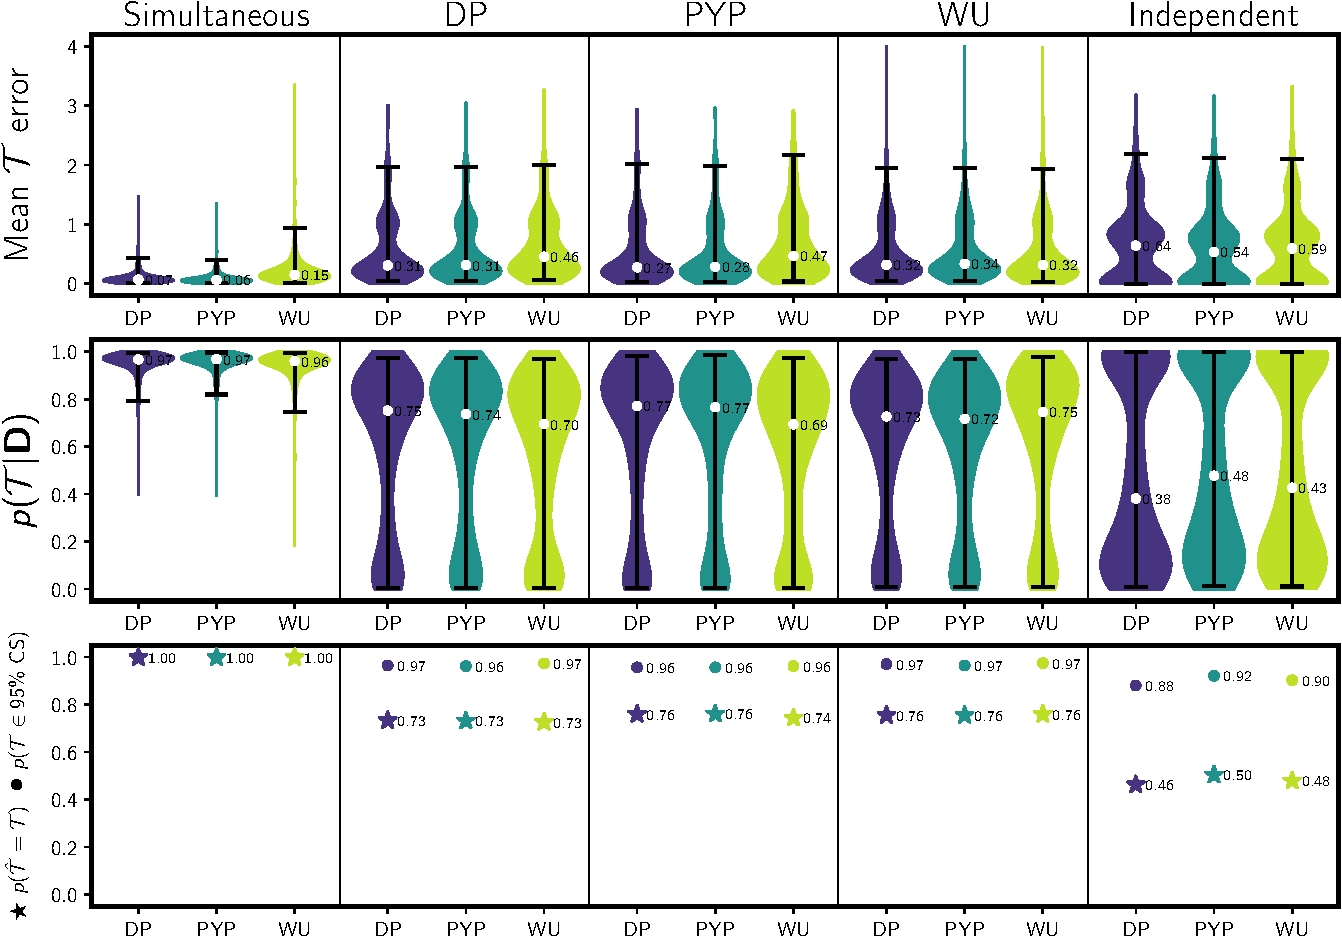
\includegraphics[width=\textwidth,height=\textheight,keepaspectratio]{../images/from-project-repo/model-performance-violin-cropped.pdf}
        \captionsetup{listformat=figList}
        \caption{
        Comparing the models' ability to estimate the divergence model.
        Each column of plots compares the performance of the Dirichlet process
        (DP), Pitman-Yor process (PYP) and weighted-uniform (WU) models when
        analyzing 720 \datasets simulated under the (from left-to-right)
        simultaneous-divergence, DP, PYP, WU, and independent-divergences
        model. 
        Mean \etimesets error is the mean partition distance
        of the posterior samples from the true
        divergence model (\etimesets),
        $p(\etimesets \given \alldata)$ is the posterior probability
        of the true divergence model,
        $p(\etimesets \given \alldata)$ is the posterior probability of the
        true divergence model,
        and
        $p(\etimesets \in \textrm{95\% CS})$ is the proportion of simulation
        replicates for which he true \etimesets is included in the 95\%
        posterior credibility set of divergence models.
        The bars overlaying the violin plots show the interval between the
        2.5\% and 97.5\% percentiles, and the white dot is the median.
        We generated the plot using matplotlib Version 3.1.3
        \citep{matplotlib}.
        }
        \label{fig:modelperformancegrid}
    \end{center}
\end{figure}

\begin{figure}[htbp]
    \begin{center}
        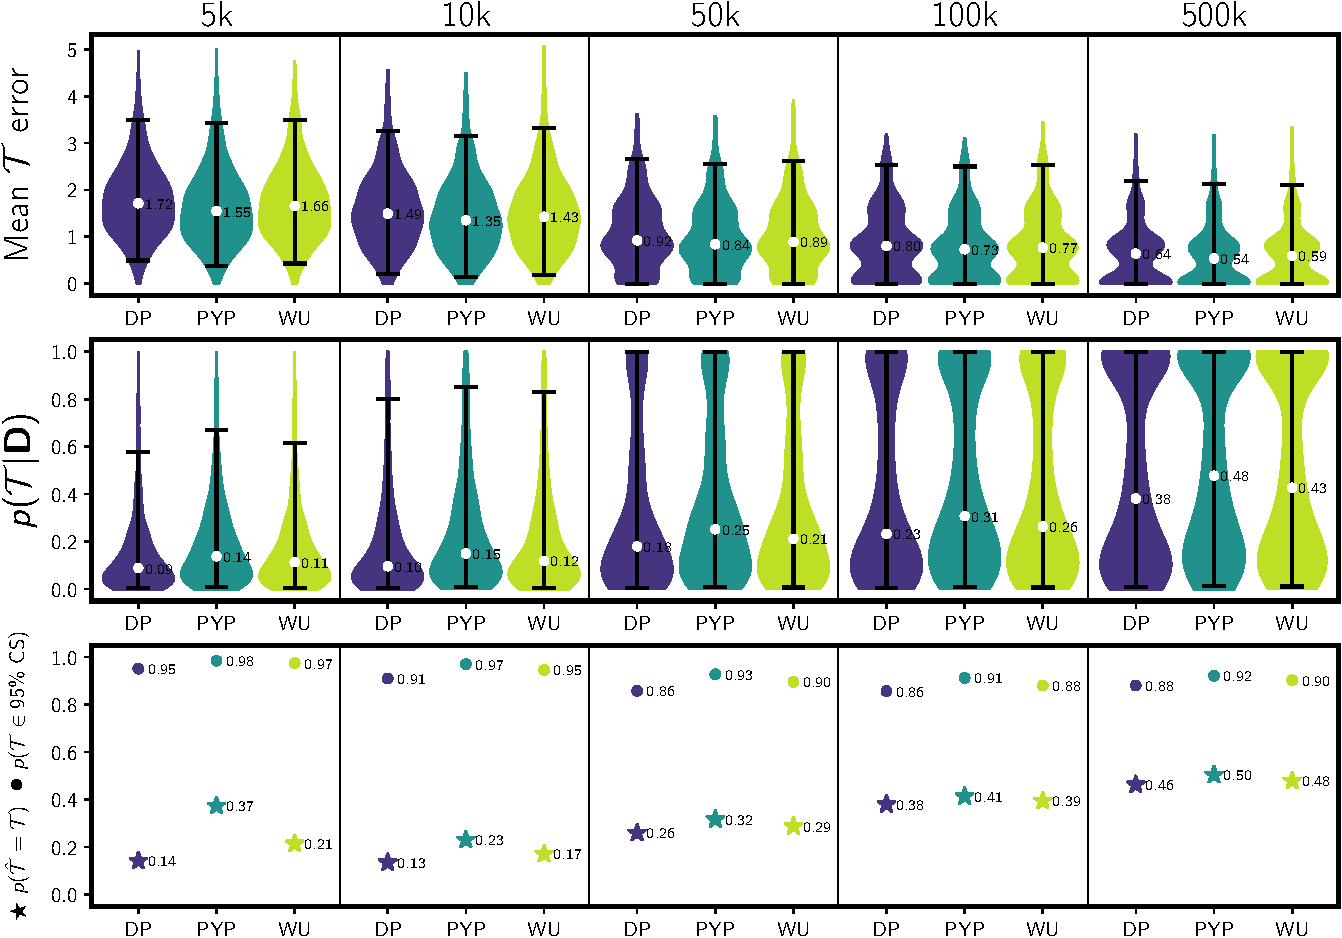
\includegraphics[width=\textwidth,height=\textheight,keepaspectratio]{../images/from-project-repo/nchars-model-performance-violin-cropped.pdf}
        \captionsetup{listformat=figList}
        \caption{
        Comparing the models' ability to estimate the independent-divergence
        model as the \dataset size increases.
        Each column of plots compares the performance of the Dirichlet process
        (DP), Pitman-Yor process (PYP) and weighted-uniform (WU) models when
        analyzing 720 \datasets with 5,000 to 500,000 characters simulated
        under the independent-divergences model.
        Mean \etimesets error is the mean partition distance
        of the posterior samples from the true
        divergence model (\etimesets),
        $p(\etimesets \given \alldata)$ is the posterior probability
        of the true divergence model,
        $p(\etimesets \given \alldata)$ is the posterior probability of the
        true divergence model,
        and
        $p(\etimesets \in \textrm{95\% CS})$ is the proportion of simulation
        replicates for which he true \etimesets is included in the 95\%
        posterior credibility set of divergence models.
        The bars overlaying the violin plots show the interval between the
        2.5\% and 97.5\% percentiles, and the white dot is the median.
        We generated the plot using matplotlib Version 3.1.3
        \citep{matplotlib}.
        }
        \label{fig:modelperformancebysize}
    \end{center}
\end{figure}

Summary Statistics
Before looking at the results here are some summary statistics that we need to 
understand in order to interpret the results. Coverage or credible sites is the probability
of the number events within the credible sites. The probability of estimated number 
of events equal to the true number of events which basicially tells us how often we 
are right. Median posterior probability is the true number of events given the data 
and this summary statistics tells us how much support we have for the correct answer.
Root mean square error quantifies how much error is there and comparing the true 
value to the estimate value. 
Hyper Parameter Estimation 
We are going to look how well the hyper parameters are estimated. Dirichlet
prior has as a single parameter called concentration parameter that tells how cluster 
the process is. The result of estimated concentration versus true concentration plot
shows that the true value is within 95\% credible sites. Pitman-Yor prior has two 
parameters(concentration parameter and discount parameter) the estimated value of 
concentration versus the true value indicates that the true is also within 95\%
credible sites. The Uniform prior has split weight and the result of estimated value 
versus the true value shows the true value is little less comparing to the other two 
priors but it's still within 94\% credible sites.
In this study, we are interested in divergence time and sharing divergence time and 
everything else is nuisance parameters. For both divergence time and sharing divergence time 
estimation we analyzed data with constant sites and without constant sites. First, we are going 
to look at the results of divegence time estimation with constant sites. The models which generated 
the data in rows and columns represent the models under which the data is analyzed. The true divergene 
time is on x-axis and the estimated divergence time is on y-axis. The results of true divergence 
time versus estimated divengence time show that all the three models (DP, PYP, and SW) performed
equally well with very similiar coverage around 95\%. Except for independent all others have truths 
contianed in within that 95\% credible interval. Independent is little lower because it's evolving 
indepdently and we are not modeling that way. We haven't observed any patterns that differiate
these 3 models. Root mean square errors are very similiar across all the models as well. 
With variable sites only there are more variation in estimates when throwing the invariable 
sites which contain lot of information and when we use them we have much more presicion in estimates
than ingoring them. All 10 pairs diverge spontatnous recently causing some MCMC issues and there 
are very few variable sites all 10 pairs diverged recently. Basicailly there is discrepency bewtween 
gene divergence and population divergence which is the largest at the most recent divergent times.
Comparing the true number of events with estimated number of events among all the sites. The true 
divergence time ranges from 1 to 10 and 1 they all share the divergence time and 10 they all 
diverged independently. The true number of events is the one has the higest posterior probability.
We have 520 replicates and the grid shows how many of them dall in each cell. The result shows 
that the data geenrated under PYP and analyzed under PYP. There are 88 datasets for which the true 
number of divergence is 5 and 76 out of those 88 got the that number correctly. 11 out of 88 
estimated 4 diverngence times and 1 out of 88 estimated 3 divergence time. 
The results for two constraint models all the 3 models under which the data is analyzed show that 
half of the time there are 10 indepedent divergence times for the datasets that is generated under 
indepdent model. The models are doing very well and they got half of time the correct asnwer. The 
ones got wrong are not that far away from the true and they are 8 or 9 event. PYP seems like 
doing little better in terms of how often ge tthe correct answer and also the confident in that 
correct asnwer. The median posterior probability for k=10 getting the correct answer
given the data is 47\% and it's little lower for the other models. The scenario of co-divergence
is an easy scenario and it has the proability of 1 for true number of event versus estimated number of 
event. When the true 1 the models are doing very well estimating the number of divergence time. But 
when the truth is 10 everything is diverging indepdently then it's more difficult scenario for 
modles to handle. Therefore, there is variation in the results. 
The results of true number of events versus estimated number of events among variable sites. The
constant sites are very informative and without invariable sites, the median posterior probability
which is the correct answer is much lower. But the covarage is unaffacted because the 
likelihood for the missing invariable characters is corrected in Ecoevolity. PYP is doing better when 
dealing with the most difficult scenario all the 10 pairs are diverging independetly as well. Both in
terms of covrage and getting the correct answer is much higher than the other two models. 

\subsubsection{Comparing DP, PYP, and \wunif across \dataset sizes}

% #### 
% Nuisane Parameters


\subsection{Empirical application?}


\section{Discussion}


\section{Acknowledgments}

We thank \ldots
This work was supported by funding provided to JRO from the National Science
Foundation (NSF grant number DEB 1656004).
The computational work was made possible by the Auburn University (AU) Hopper
Cluster supported by the AU Office of Information Technology
and
a grant of high-performance computing resources and technical support from the
Alabama Supercomputer Authority.
This paper is contribution number \highLight{XXX} of the Auburn University
Museum of Natural History.


%TC:ignore

\bibliographystyle{evolution}
\bibliography{references}


\iflinenumbers{
\end{linenumbers}
}{}


%%%%%%%%%%%%%%%%%%%%%%%%%%%%%%%%%%%%%%%%%%%%%%%%%%%%%%%%%%%%%%%%%%
%% SUPPORTING INFO %%%%%%%%%%%%%%%%%%%%%%%%%%%%%%%%%%%%%%%%%%%%%%%
\newpage
\setcounter{figure}{0}
\setcounter{table}{0}
\setcounter{page}{1}
\setcounter{section}{0}

\singlespacing

\section*{Supporting Information}
\hangindent=1cm
\noindent Title: \msTitle

\bigskip
{\noindent Authors: \msAuthor}

\newpage
\singlespacing

\input{si-body.tex}
\clearpage

\input{si-tables.tex}
\clearpage

\begin{figure}[htbp]
    \begin{center}
        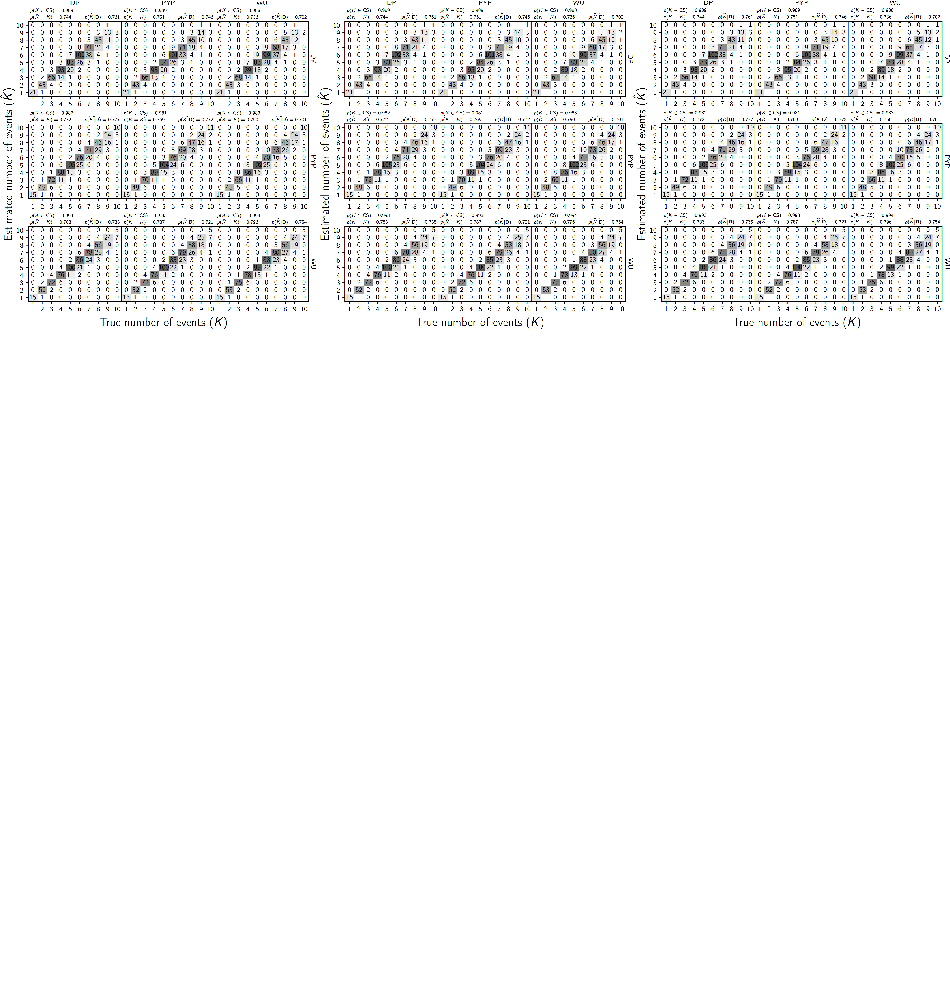
\includegraphics[width=\textwidth,height=\textheight,keepaspectratio]{../images/from-project-repo/infer-columns-by-data-rows-nevents-cropped-rasterized.pdf}
        \captionsetup{name=Figure S, labelformat=noSpace, listformat=sFigList}
        \caption{
        The models perform similarly in estimating the number of divergence
        events.
        Each plot shows the results for 720 \datasets
        simulated under the
        DP (top row),
        PYP (middle row),
        or
        WU (bottom row)
        and analyses using the
        DP (left column),
        PYP (middle column),
        or
        WU (right column).
        The number of \datasets that fall within each possible cell of true
        versus estimated numbers of events is shown, and cells with more
        \datasets are shaded darker.
        % The estimates are based on the number of events with the maximum
        % \textit{a posteriori} (MAP) probability.
        Above each plot is
        the proportion of \datasets for which the number of events with the largest
        posterior probability matched the true number of events---$p(\hat{\nevents}
        = \nevents)$,
        the median posterior probability of the correct number of events across all
        \datasets---$\widetilde{p(\nevents|\alldata)}$, and
        the proportion of \datasets for which the true number of events was
        included in the 95\% credible set---$p(\nevents \in
        \textrm{CS})$.
        We generated the plot using matplotlib Version 3.1.3
        \citep{matplotlib}.
        }
        \label{fig:neventsgrid}
    \end{center}
\end{figure}

\begin{figure}[htbp]
    \begin{center}
        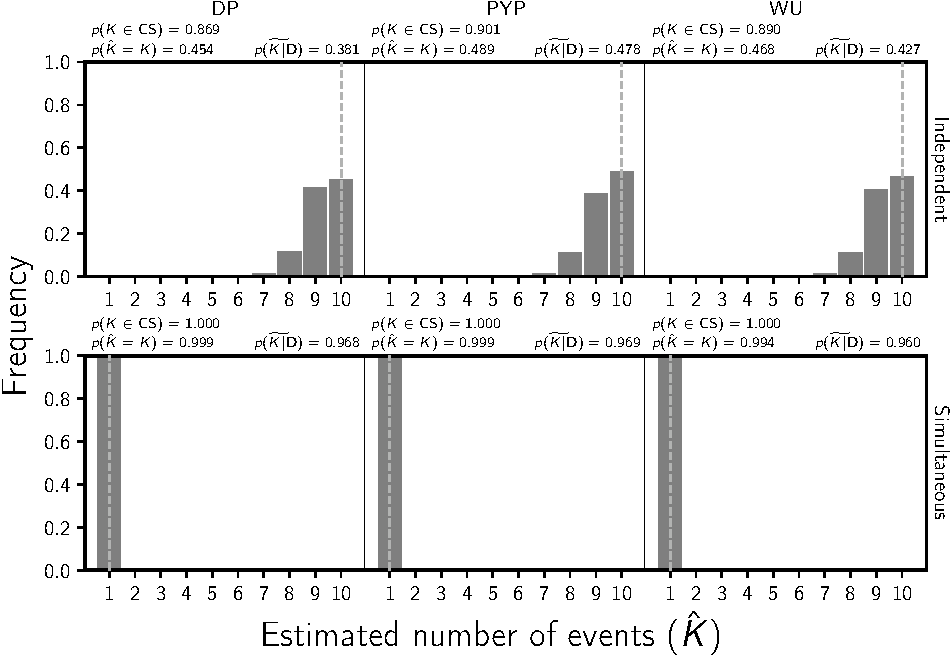
\includegraphics[width=\textwidth,height=\textheight,keepaspectratio]{../images/from-project-repo/infer-columns-by-fixed-rows-nevents-cropped.pdf}
        \captionsetup{name=Figure S, labelformat=noSpace, listformat=sFigList}
        \caption{
        The PYP (middle column) model performs better than the DP (left column)
        and WU (right column) models when analyzing simulated \datasets for
        which all 10 population pairs diverged independently (top row).
        All three models almost always correctly infer a single shared
        divergence event with high confidence when analyzing simulated
        \datasets for which that is true (bottom row).
        Each plot shows the results for 720 \datasets.
        Above each plot is
        the proportion of \datasets for which the number of events with the largest
        posterior probability matched the true number of events---$p(\hat{\nevents}
        = \nevents)$,
        the median posterior probability of the correct number of events across all
        \datasets---$\widetilde{p(\nevents|\alldata)}$, and
        the proportion of \datasets for which the true number of events was
        included in the 95\% credible set---$p(\nevents \in
        \textrm{CS})$.
        We generated the plot using matplotlib Version 3.1.3
        \citep{matplotlib}.
        }
        \label{fig:neventsfixedcomparison}
    \end{center}
\end{figure}


%TC:endignore

\end{document}
